\begin{frame}
    \resizebox{\linewidth}{!}{
        \begin{minipage}[t]{1.1\textwidth}
            \begin{itemize}
                \item<1-> Bare-metal programming
                    \begin{itemize}
                        \item ``Infinite loop''
                        \item Little or no software overhead
                        \item High control of hardware
                        \item Single-purpose or simple applications, hardware-dependent
                        \item Strict timing (e.g. motor control)
                    \end{itemize}
                \item<2-> \ac{rtos}
                    \begin{itemize}
                        \item Scheduler overhead
                        \item More powerful microcontroller required
                        \item High control of hardware
                        \item Multithreading, some common libraries
                        \item Multiple tasks: networking, user interface, etc.
                    \end{itemize}
                \item<3-> Embedded \ac{gpos}
                    \begin{itemize}
                        \item Large overhead (scheduler, memory management, background tasks, \ldots)
                        \item Microprocessor usually required (and often external \acs{ram} and \acs{nvm})
                        \item Low direct control of hardware (files or abstraction layers)
                        \item Multiple threads and processes, many common libraries
                        \item Multiple complex tasks: networking, file system, graphical interface, \ldots
                    \end{itemize}
            \end{itemize}
        \end{minipage}%
        \begin{minipage}[t]{0.35\textwidth}
            \onslide<1->{
                \begin{figure}
                    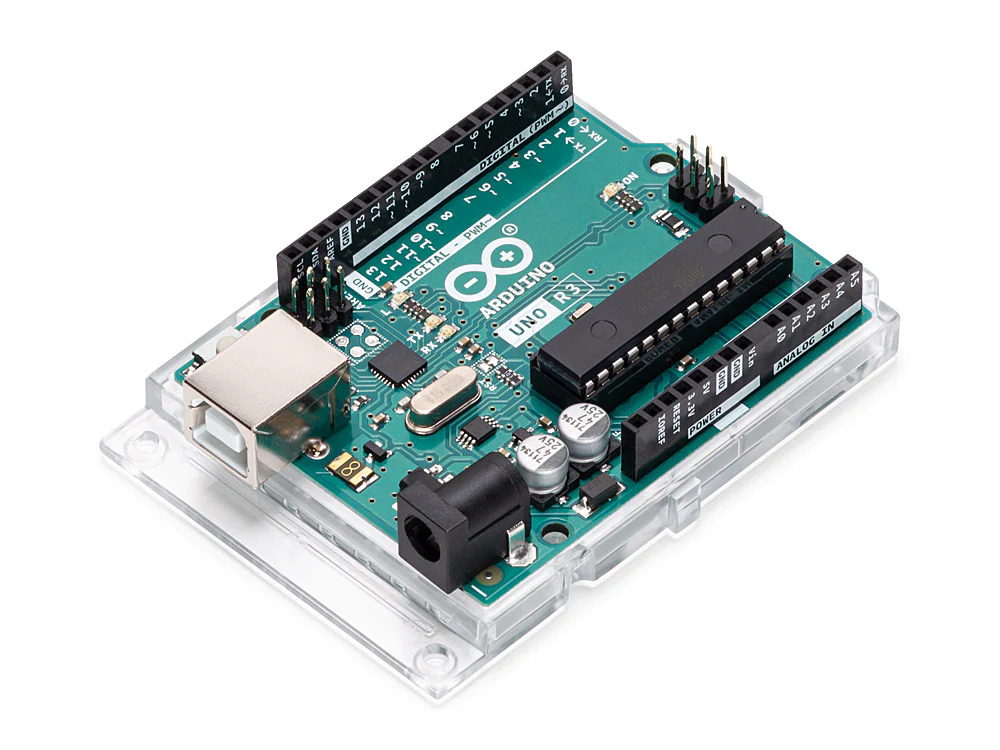
\includegraphics[height=2cm]{microcontroller/arduino/boards/uno.jpg}
                    \caption{\href{https://store.arduino.cc/products/arduino-uno-rev3}{Arduino\textregistered{} Uno}}
                \end{figure}
            }
            \onslide<2->{
                \begin{figure}
                    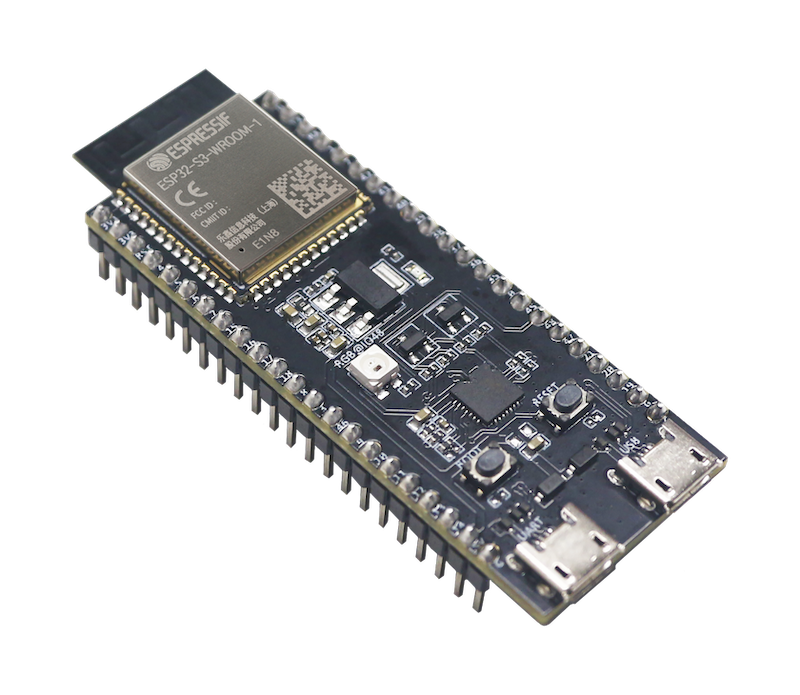
\includegraphics[height=2cm]{microcontroller/boards/esp32-s3-devkitc-1-v1-isometric.png}
                    \caption{\href{https://docs.espressif.com/projects/esp-idf/en/latest/esp32s3/hw-reference/esp32s3/user-guide-devkitc-1.html}{ESP32-S3 DevKitC-1}}
                \end{figure}
            }
            \onslide<3->{
                \begin{figure}
                    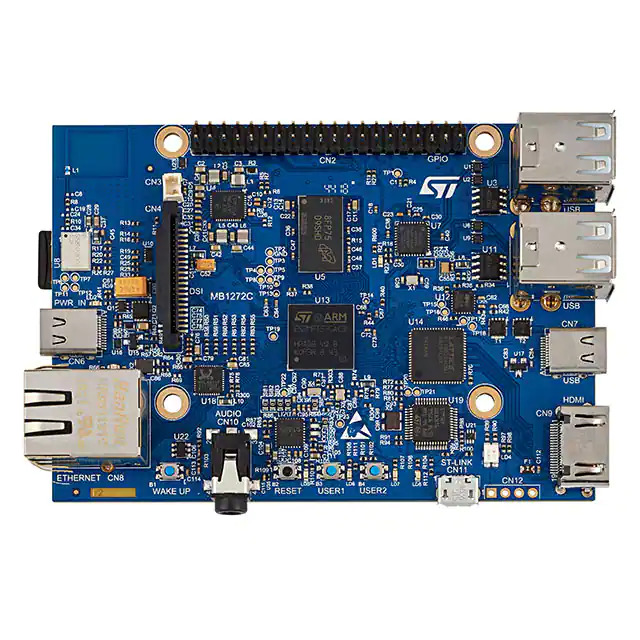
\includegraphics[height=2cm]{microcontroller/boards/stm32mp157d-dk1.jpg}
                    \caption{\href{https://www.st.com/en/evaluation-tools/stm32mp157d-dk1.html}{STM32MP157D-DK1}}
                \end{figure}
            }
        \end{minipage}
    }
\end{frame}

\begin{frame}
    \begin{figure}
        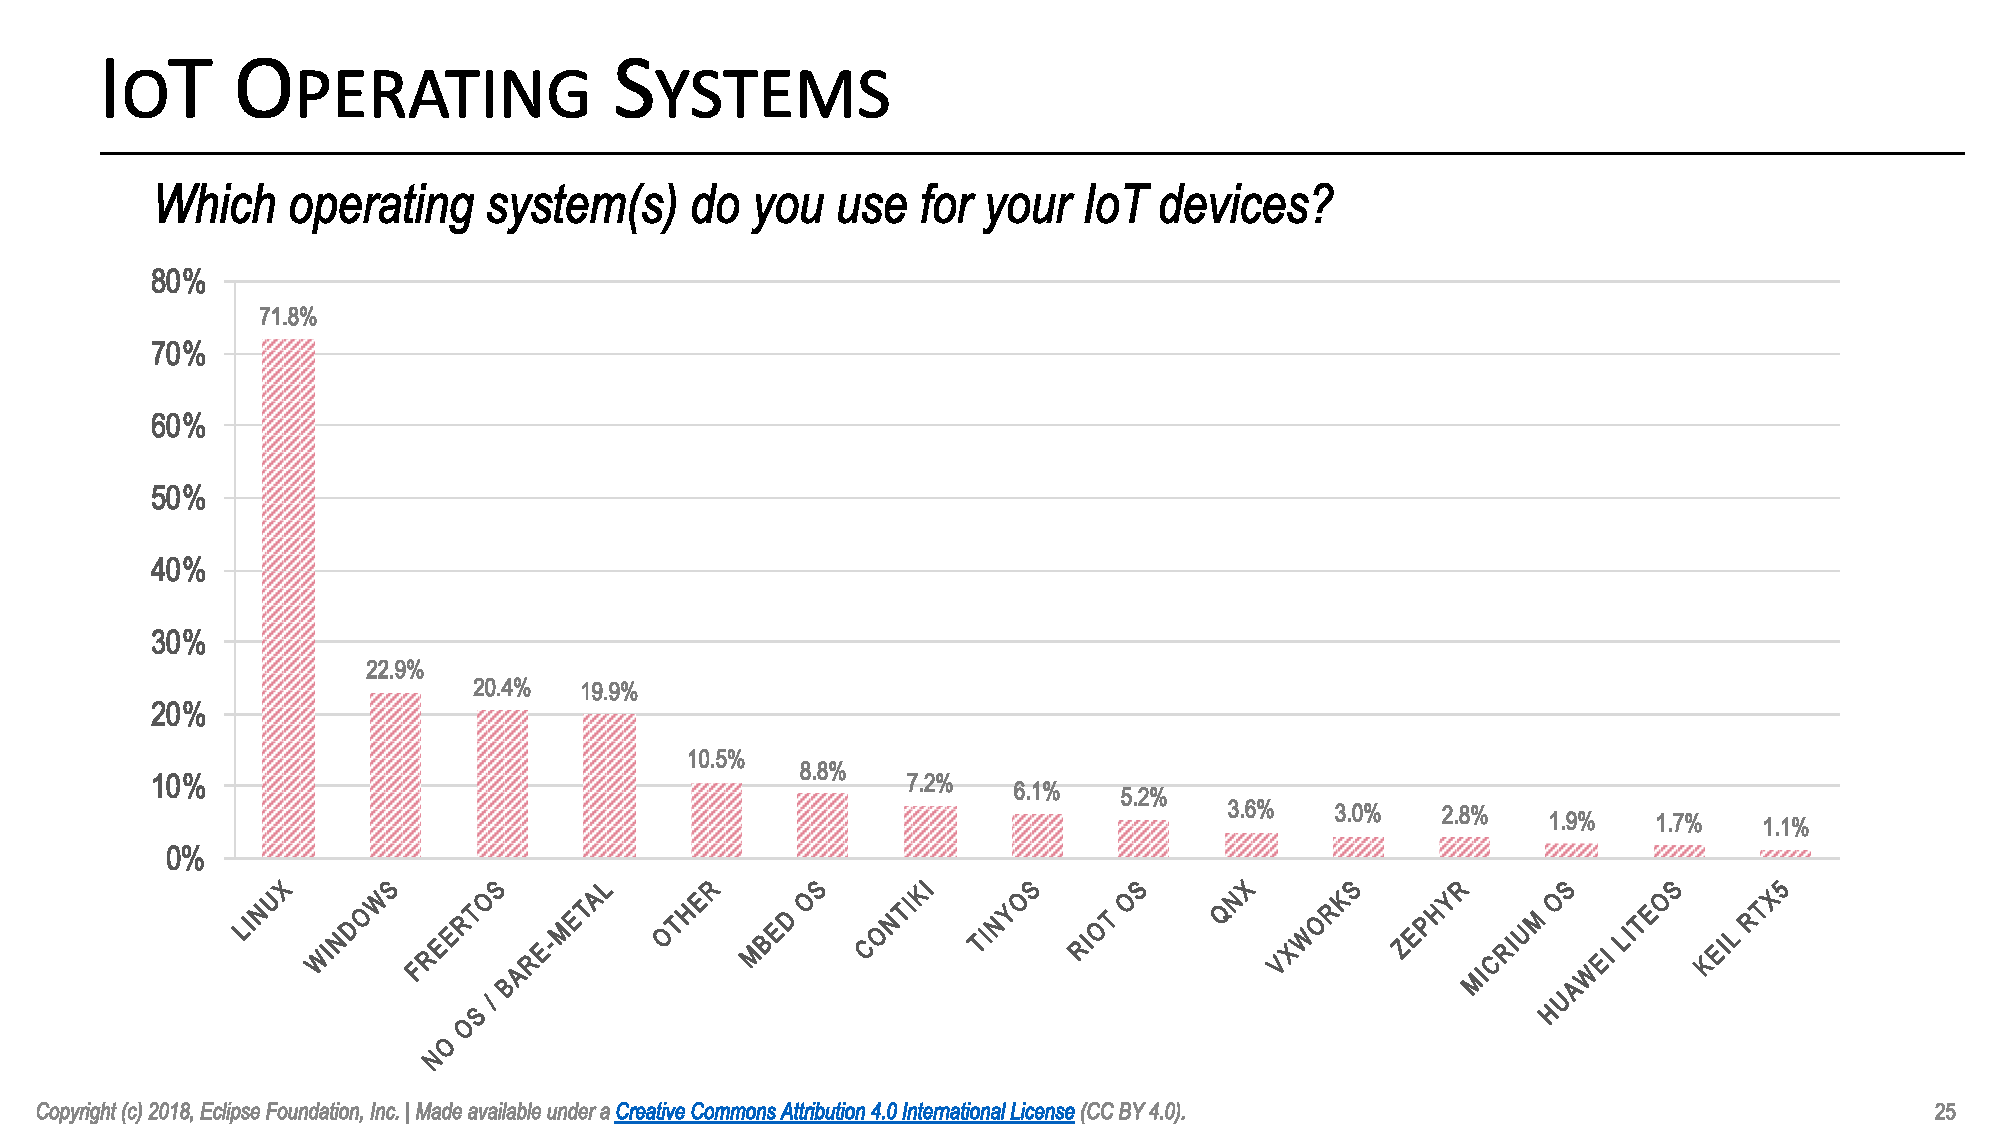
\includegraphics[width=\textwidth]{microcontroller/iot-developer-survey-2018-os.pdf}
        \caption{\href{https://iot.eclipse.org/community/resources/iot-surveys/assets/iot-developer-survey-2018.pdf}{Eclipse \glsentrytext{iot} Developer Survey}: \glsentrydesc{os}s}
    \end{figure}
\end{frame}